\documentclass[aspectratio=169]{beamer}
%
% Choose how your presentation looks.
%
% For more themes, color themes and font themes, see:
% http://deic.uab.es/~iblanes/beamer_gallery/index_by_theme.html
%
\mode<presentation>
{
  \usetheme{default}      % or try Darmstadt, Madrid, Warsaw, ...
  \usecolortheme{default} % or try albatross, beaver, crane, ...
  \usefonttheme{default}  % or try serif, structurebold, ...
  \setbeamertemplate{navigation symbols}{}
  \setbeamertemplate{caption}[numbered]
} 

\usepackage[english]{babel}
\usepackage[utf8]{inputenc}
\usepackage[T1]{fontenc}
\usepackage{graphicx}
\usepackage{booktabs}

\usepackage[binary-units]{siunitx}
\usepackage{hyperref}
\newcommand{\gbs}{\si[per-symbol = \text{~div~}]{\gibi\byte\per\second}}

\title[Your Short Title]{Benchmarking}
\author{You}
% \institute{Where You're From}
\date{Date of Presentation}

\begin{document}

\begin{frame}
  \titlepage
\end{frame}

\section{Introduction}

\subsection{System}
\begin{frame}{System Topology}
\begin{figure}
    \centering
    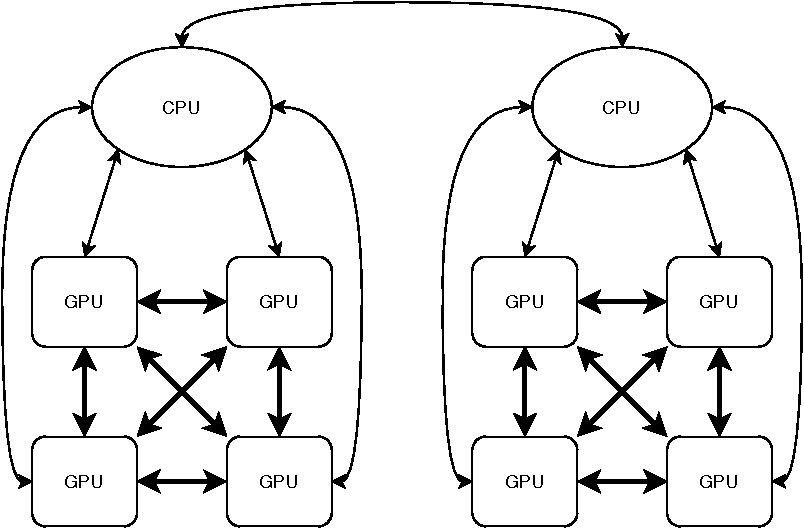
\includegraphics[height=.75\textheight]{figs/kleurplaat-topology.pdf}
    \caption{System topology}
    \label{fig:topology}
\end{figure}
    
\end{frame}

\begin{frame}{AMD Radeon Instinct MI50}

\begin{columns}
\begin{column}{0.5\textwidth}
    \begin{itemize}
    \item Vega 20 GLXT
    \item Wavefront size: 64
    \item 32GB memory
    \item 16kB L1 cache (per CU)
    \item 60 compute units
    \end{itemize}
\end{column}
\begin{column}{0.5\textwidth}  %%<--- here
    \begin{center}
     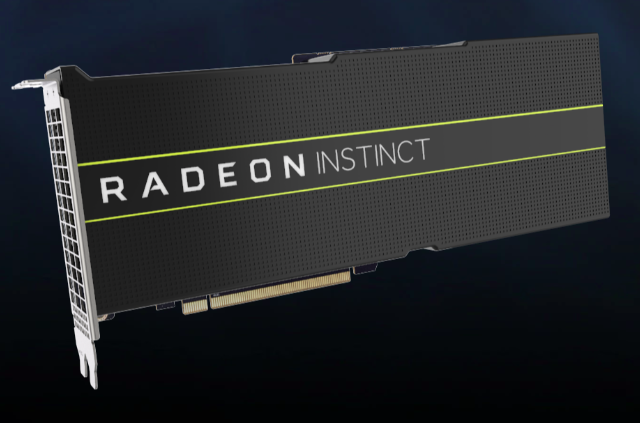
\includegraphics[width=1\textwidth]{figs/mi50.png}
     \end{center}
\end{column} 
\end{columns}

\end{frame}

\section{Benchmarks}
\begin{frame}{Benchmarking}
    \begin{itemize}
    \item Three benchmarks to show GPU performance
        \begin{itemize}
            \item SHOC L0
            \item rocm-bandwidth-test
            \item Multi-GPU vector add
        \end{itemize}
    \end{itemize}
    
\end{frame}

\subsection{SHOC}
\begin{frame}{Scalable HeterOgeneous Computing (SHOC)}
    \begin{itemize}
        \item Benchmark suite for Heterogeneous Computing
        \item CUDA, openCL and MPI backends
        \item Level 0 provides low level benchmarks
    \end{itemize}
\end{frame}

\begin{frame}{SHOC: Performance}
\begin{table}[]
    \centering
    \begin{tabular}{l|r|r}
Benchmark & Measured & Theoretical Max \\
\hline
readGlobalMemoryCoalesced &	- \gbs & - \gbs \\
readGlobalMemoryUnit      & - \gbs & - \gbs \\
\hline
maxdpflops                &  - GFLOPS    & - GFLOPS    \\
maxspflops                &  - GFLOPS    & - GFLOPS    \\ 
\hline
\end{tabular}
    \caption{SHOC performance numbers for a }
    \label{tab:SHOCnumbers}
\end{table}
\end{frame}

\subsection{ROCm benchmark test}
\begin{frame}{RadeonOpenCompute (ROCm) bandwidth test}
    \begin{itemize}
        \item Part of the ROCm platform
        \item Support for Host-to-Host, Host-to-Device, Device-to-Device
    \end{itemize}
\end{frame}

\begin{frame}{ROCm benchmark test: Performance}
\begin{table}[]
    \centering
    \begin{tabular}{l|r|r}
Benchmark & Measured & Theoretical Max \\
\hline
Host-to-Device (same island)      & - \gbs & - \gbs \\
Device-to-Device (same island)    & - \gbs & - \gbs \\
\hline
Host-to-Device (across islands)      & - \gbs & - \gbs \\
Device-to-Device (across islands) & - \gbs & - \gbs \\
\hline
\end{tabular}
    \caption{SHOC performance numbers for a }
    \label{tab:ROCmnumbers}
\end{table}
\end{frame}

\subsection{Multi-GPU vector add}
\begin{frame}{Multi-GPU vector add}
    \begin{itemize}
        \item Multi-GPU using openMP?
    \end{itemize}
\end{frame}

\begin{frame}{Multi-GPU vector add: Performance}
\begin{table}[]
    \centering
    \begin{tabular}{l|r|r}
Benchmark & Measured & Theoretical Max \\
\hline
Single GPU      & - & - \\
Multi GPU (same islands) & - & - \\
Multi GPU (across islands) & - & - \\
\hline
\end{tabular}
    \caption{SHOC performance numbers for a }
    \label{tab:vec-add-numbers}
\end{table}
\end{frame}

\section{Conclusion}
\begin{frame}{Conclusion?}
    \begin{itemize}
        \item Some closing remarks
        \item Encourage participants to try the benchmarks on the machine.
        \item Hands on examples can be found at ...
    \end{itemize}
\end{frame}


\begin{frame}{Useful Resources}
    \begin{itemize}
        \item ROCm: \url{https://rocm.github.io/}
        \item SHOC: \url{https://github.com/vetter/shoc/wiki}
        \item MI50: \url{https://www.amd.com/system/files/documents/radeon-instinct-mi50-datasheet.pdf}
    \end{itemize}
\end{frame}


\end{document}
